\paragraph[QuizziPedia::Front-End::Controllers\\::ProfileManagementController]{QuizziPedia::Front-End::Controllers::ProfileManagementController}
\begin{figure} [ht]
	\centering
	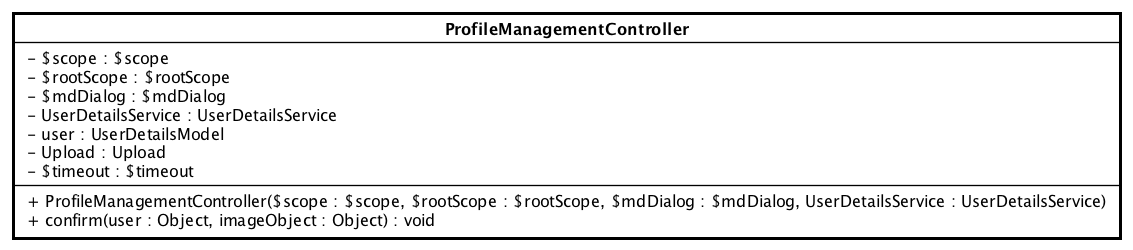
\includegraphics[scale=0.45]{UML/Classi/Front-End/QuizziPedia_Front-end_Controller_ProfileManagementController.png}
	\caption{QuizziPedia::Front-End::Controllers::ProfileManagementController}
\end{figure} \FloatBarrier
\begin{itemize}
	\item \textbf{Descrizione}: questa classe permette di gestire il profilo personale di un utente; 
	\item \textbf{Utilizzo}: fornisce le funzionalità all'utente per poter gestire i propri dati;
	\item \textbf{Relazione con altre classi}:
	\begin{itemize}
		\item \textbf{IN \texttt{ProfileManagementModelView}}: classe di tipo \textit{modelview\ped{G}} la cui istanziazione è contenuta all'interno della variabile di ambiente \$scope di \textit{Angular\ped{G}}. All'interno di essa sono presenti le variabili e i metodi necessari per il \textit{Two-Way Data-Binding\ped{G}} tra la \textit{view\ped{G}} \texttt{ProfileManagementView} e il \textit{controller\ped{G}} \texttt{ProfileManagementController};
		\item \textbf{IN \texttt{UserDetailsService}}: questa classe permette di ottenere i dati personali degli utenti;
		\item \textbf{IN \texttt{UserDetailsModel}}: questa classe rappresenta il tipo dell'utente autenticato della pagina.
	\end{itemize}
	\item \textbf{Attributi}:
	\begin{itemize}
		\item \texttt{-} \texttt{\$scope: \$scope} \\
		Campo dati contenente un riferimento all'oggetto \$scope creato da \textit{Angular\ped{G}}, viene utilizzato come mezzo di comunicazione tra il \textit{controller\ped{G}} e la \textit{view\ped{G}}. Contiene gli oggetti che definiscono il \textit{model\ped{G}} dell'applicazione;
		\item \texttt{-} \texttt{\$rootScope: \$rootScope} \\
		Campo dati contenente il riferimento all'oggetto globale \$rootScope creato da \textit{Ang-\\ular\ped{G}}. Viene utilizzato per rendere accessibile a tutti i \textit{controller\ped{G}} e a tutte le \textit{view\ped{G}} l'oggetto \texttt{UserDetailsModel};
		\item \texttt{-} \texttt{\$mdDialog: \$mdDialog} \\
		Campo dati contenente un riferimento al servizio della libreria \textit{Material for Angular\ped{G}} che permette di creare delle componenti a pop-up;		
		\item \texttt{-} \texttt{UserDetailsService: UserDetailsService}: \\
		Campo dati contenente un riferimento al servizio che si occupa della gestione delle informazioni legate agli utenti;
		\item \texttt{-} \texttt{user: UserDetailsModel}: \\
		Oggetto di tipo \texttt{UserDetailsModel}. Viene mantenuto all'interno del \$rootScope; 
		\item \texttt{-} \texttt{Upload: Upload} \\
		Campo dati contenente un riferimento alla libreria \textit{ng-file-upload\ped{G}} necessaria per il caricamento della foto profilo dell'utente;
		\item \texttt{-} \texttt{\$timeout: \$timeout} \\
		Campo dati contenente il riferimento all'oggetto globale \$timeout creato da \textit{Angular\ped{G}}. 
		Il valore di ritorno di una chiamata alla funzione di \$timeout è una \textit{promise\ped{G}}, la quale sarà risolta quando avverrà il ritardo e la funzione di \$timeout sarà eseguita; 
	\end{itemize}
	\item \textbf{Metodi}:
	\begin{itemize}
		\item \texttt{+} \texttt{ProfileManagementController(\$scope: \$scope, \$rootScope: \$rootScope,\\ \$mdDialog: \$mdDialog, UserDetailsService: UserDetailsService)} \\
		Metodo costruttore della classe. \\
		\textbf{Parametri}:
		\begin{itemize}
			\item \texttt{\$scope: \$scope} \\
			Parametro contenente un riferimento all'oggetto \$scope creato da \textit{Angular\ped{G}}. Viene utilizzato come mezzo di comunicazione tra il \textit{controller\ped{G}} e la \textit{view\ped{G}}. Contiene gli oggetti che definiscono il \textit{viewmodel\ped{G}} e il \textit{model\ped{G}} dell'applicazione;
			\item \texttt{\$rootScope: \$rootScope} \\
			Parametro contenente il riferimento all'oggetto globale \$rootScope creato da \textit{Ang-\\ular\ped{G}}. Viene utilizzato per rendere accessibile a tutti i \textit{controller\ped{G}} e a tutte le \textit{view\ped{G}} l'oggetto \texttt{UserDetailsModel}. In questo caso viene utilizzato per aggiornare in \$rootScope l'oggetto che rappresenta l'utente autenticato all'interno dell'applicazione;
			\item \texttt{\$location: \$location} \\
			Parametro contenente un riferimento al servizio creato da \textit{Angular\ped{G}} che permette di accedere alla barra degli indirizzi del \textit{browser\ped{G}}, i cambiamenti all'URL nella barra degli indirizzi si riflettono in questo oggetto e viceversa;
			\item \texttt{\$mdDialog: \$mdDialog} \\
			Parametro contenente un riferimento al servizio della libreria \textit{Material for Angular\ped{G}} che permette di creare delle componenti a pop-up;
			\item \texttt{UserDetailsService: UserDetailsService} \\
			Parametro contenente un riferimento al servizio che si occupa della gestione delle informazioni legate all'utente;
			\item \texttt{Upload: Upload} \\
			Parametro contenente un riferimento alla libreria \textit{ng-file-upload\ped{G}} necessaria per il caricamento della foto profilo dell'utente;
			\item \texttt{\$timeout: \$timeout} \\
			Parametro contenente il riferimento all'oggetto globale \$timeout creato da \textit{Angular\ped{G}}. 
			Il valore di ritorno di una chiamata alla funzione di \$timeout è una \textit{promise\ped{G}}, la quale sarà risolta quando avverrà il ritardo e la funzione di timeout sarà eseguita. 
		\end{itemize}
		\item \texttt{+} \texttt{confirm(user: Object, imageObject: Object): void} \\
		Metodo che gestisce l'evento click sul pulsante di conferma modifica. Aggiorna, in caso di modifiche, l'oggetto locale \texttt{UserDetailsModel}. Inoltre, utilizzando il metodo dell'\texttt{UserDetailsService}, aggiorna anche nel \textit{server\ped{G}} i dati dell'utente.
	\end{itemize}
\end{itemize}

